%%%%%%%%%%%%%%%%%%%%%%%%%%%%%%%%%%%%%%%%%%%%%%%%%%%%%%%%%%%%%%%%%%%%%
% Author: Deepak Gupta
% 
% This is an example of a very complete CV using the 'moderncv' package
% and the 'timeline' package. For more information on those, please
% access: 
% https://www.ctan.org/tex-archive/macros/latex/contrib/moderntimeline
% https://www.ctan.org/tex-archive/macros/latex/contrib/moderncv
%%%%%%%%%%%%%%%%%%%%%%%%%%%%%%%%%%%%%%%%%%%%%%%%%%%%%%%%%%%%%%%%%%%%%

\documentclass[12pt, a4paper, sans]{moderncv}

\moderncvstyle{classic}
\moderncvcolor{ blue} 
\usepackage[utf8]{inputenc}
\usepackage[scale=0.90]{geometry}    % Width of the entire CV
%\geometry{left=1.5cm,right=1cm,marginparwidth=2cm,marginparsep=1.2cm,top=0.5cm,bottom=0cm}
\setlength{\hintscolumnwidth}{3.7cm} % Width of the timeline on your left
\usepackage{graphicx,xcolor,fontawesome}
%\usepackage{fontspec}
\usepackage{xcolor}
\usepackage{framed}
\usepackage{ifsym}
%\usepackage{hyperref} 
\usepackage{pdfpages/pdfpages}
\usepackage{moderntimeline/moderntimeline}
\usepackage{xpatch/xpatch}
\usepackage{color, graphicx}
\tlmaxdates{2006}{2021}              % Beginning and start of your timeline                        

\newcommand{\cvreferencecolumn}[2]{%
  \cvitem[0.8em]{}{%
    \begin{minipage}[t]{\listdoubleitemmaincolumnwidth}#1\end{minipage}%
    \hfill%
    \begin{minipage}[t]{\listdoubleitemmaincolumnwidth}#2\end{minipage}%
    }%
}

\newcommand{\cvreference}[8]{%
    \textbf{#1}\newline% Name
    \ifthenelse{\equal{#2}{}}{}{\addresssymbol~#2\newline}%
    \ifthenelse{\equal{#3}{}}{}{#3\newline}%
    \ifthenelse{\equal{#4}{}}{}{#4\newline}%
    \ifthenelse{\equal{#5}{}}{}{#5\newline}%
    \ifthenelse{\equal{#6}{}}{}{\emailsymbol~\texttt{\href{mailto:#6}{\nolinkurl{#6}}}\newline}%
    \ifthenelse{\equal{#7}{}}{}{\phonesymbol~#7\newline}
    \ifthenelse{\equal{#8}{}}{}{\mobilephonesymbol~#8}}

% List of journals that I may need to use in the bibtex file 

\def\memsai{Mem.~Soc.~Astron.~Italiana}
\definecolor{shadecolor}{RGB}{180,180,180}
\definecolor{applegreen}{rgb}{0.55, 0.71, 0.0}
\definecolor{awesome}{rgb}{1.0, 0.13, 0.32}
% Personal Information

%\name{~~~~Deepak Gupta\newline}{}


%\title{\emph{~~~~~~~~~~~~~~~~Resum\~e}}  

\address {\faHome ~\href{https://goo.gl/maps/sGwYzQNZ8oeQ2eEN8} {Gupta Bros., Lala ka Bazar,} \\ \href{https://goo.gl/maps/sGwYzQNZ8oeQ2eEN8}{Lashkar,}}{\href{https://goo.gl/maps/sGwYzQNZ8oeQ2eEN8}{Gwalior,474001 (MP), India}}{}

\phone[mobile]{\href{https://wa.me/+918982856937}{+91~89828~56937}}             
\phone[fixed]{\href{https://wa.me/+918982856937}{(0751)~~2454220}}
\email{deepakgupta1491@gmail.com}                % optional, remove / comment the line if not wanted
   % optional, remove / comment the line if not wanted
%\social[linkedin]{https://br.linkedin.com/in/maria-luiza-linhares-dantas-56408033}  % optional, remove / comment the line if not wanted    

%
\includegraphics[height=2.5cm,width=2.5cm]{frame}
\social[linkedin]{DeepakGupta1491}  % optional, remove / comment the line if not wanted
%\homepage{about.me/DeepakGuptaITM/getstarted} 
\social[github]{DeepakGupta1491}   % optional, remove / comment the line if not wanted           
%\extrainfo{\emailsymbol}

%\emaillink{mdantas.astro@gmail.com}}
%\quote{Dubitando ad veritatem parvenimus - \emph{Cicerone}}                       
%\makeatletter\renewcommand*{\bibliographyitemlabel}{\@biblabel{\arabic{enumiv}}}\makeatother

\name{~ \textbf{Deepak Gupta}}{}
\begin{document}
\href{https://sites.google.com/view/deepakguptainfy/home}
{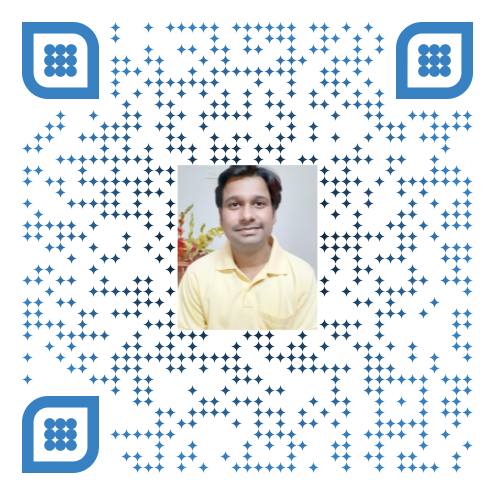
\includegraphics[height=5cm, width=5cm]{dginfy}}
\makecvtitle

\begin{tikzpicture}[remember picture, overlay]
  \node[opacity=0.14,inner sep=1pt] at (current page.center)
   {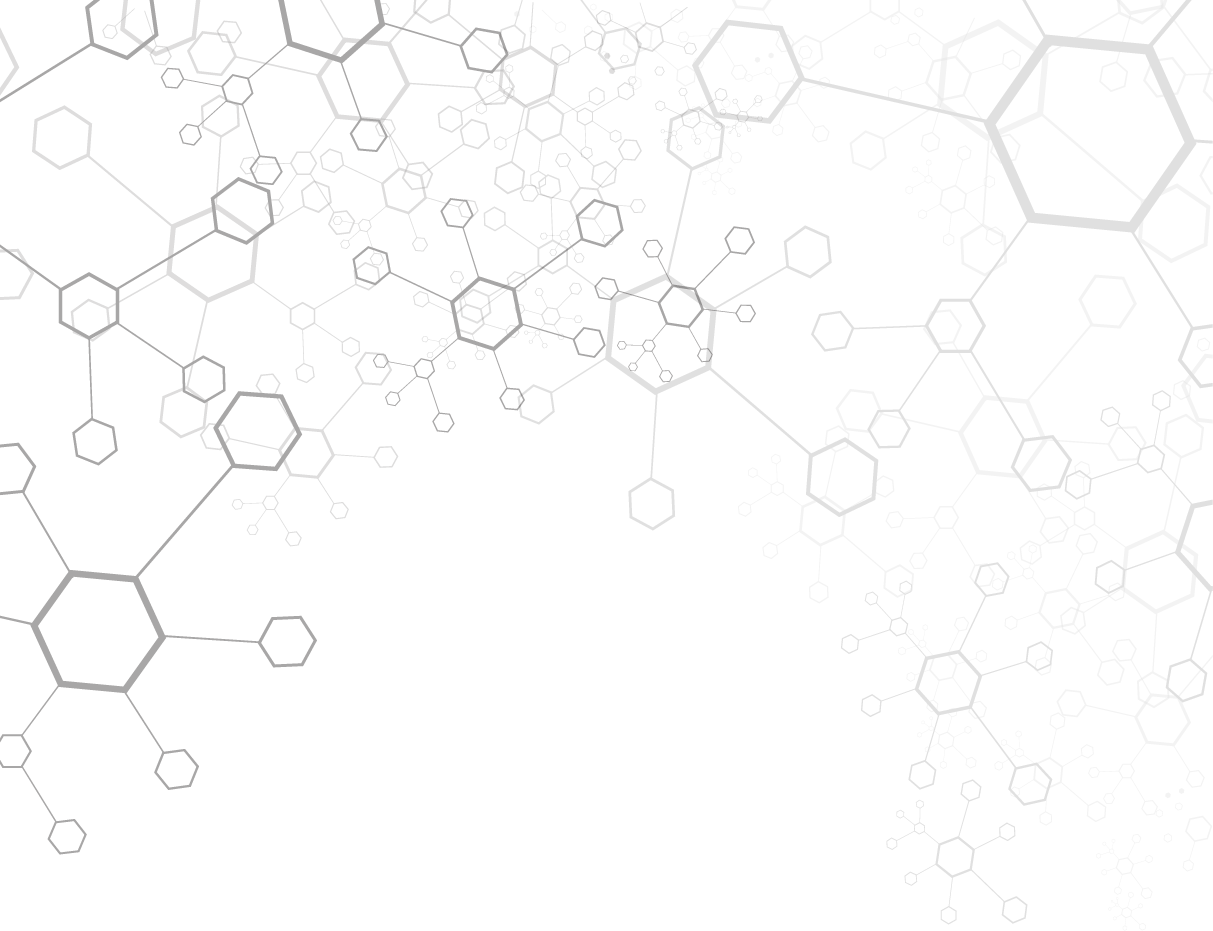
\includegraphics[width=\paperwidth,height=\paperheight]{moderncv/pngegg.png}};
  \end{tikzpicture}

\section{\textbf{Professional Summary}}
\cvitem{$\ast~~\ast~~\ast~~\ast$ }{\textbf{A results-driven professional with over 7 years+ of experience in software development and deployment, both in cloud and on-premises environments. Proficient in various domains, including Warehouse Management Systems and customized ERP solutions utilizing .NET technology. Demonstrates expertise in configuration management, continuous integration/continuous deployment (CI/CD), DevOps  and DevSecOps processes. Ensuring efficient, high-quality software product delivery. Proven track record of optimizing deployment workflows and supporting robust application lifecycle management in fast-paced, technology-driven environments. }\emph{}}
%I think my flexibility as an organization that can lead to advancement and utilizing great physical stamina and skills in organizing, sorting and categorizing to maximize the efficiency of organization. Seeking a challenging position in an engineering environment where I could add my knowledge and skills for the better productivity of the organization.
\section{\textbf{Experience}}

%IBM as DevSecOps
\tlcventry{Now}{2022}{ ~ ~ ~ Currently Associated with \href{https://www.IBM.com}{\footnote[5$\ast$]{}\color[HTML]{007CC3} \textbf{IBM}}, Noida, Work as DevSecOps Resource for Manage AWS/IBM Cloud as well as Jenkins, Tekton/Argo CI/CD.Worked on data pipeline using jenkins,python, aws databricks cluster and apache airflow.  \emph{}}{}{}{}{}{\faMapMarker ~ \textbf{\href{https://g.co/kgs/WErBq16}{IBM, Noida}} }

\medskip

\medskip


%Infosys Pvt. Ltd. as DevOps Engineer
\tlcventry{2022}{2021}{ ~~~~ Past Associated with 
\href{https://www.Infosys.com}{\footnote[4$\ast$]{}\color[HTML]{007CC3} \textbf{INFOSYS}}, Pune and Work as GCP DevOps Resource for Manage GCP Cloud as well as Cisco CI/CD Tool chain. \emph{}}{}{}{}{}{ \faMapMarker ~ \textbf{\href{https://maps.app.goo.gl/iDJug8aEkAY2sUwR8}{INFOSYS, Pune}}}

\medskip

\medskip

%SISL Infotech Pvt. Ltd. as Azure DevOps Engineer
\tlcventry{2021}{2021}{{} ~ ~ Past Associated with 
\href{https://www.sislinfotech.com}{\footnote[3$\ast$]{}\color{awesome}\textbf{SISL INFOTECH}}, Malviya Nagar, South Delhi and designated as Azure DevOps Engineer for Manages Release and Build Integration using kubernate, Jenkins, Azure DevOps Pipeline with Azure Cloud. Built and deployed Docker [POD] containers with Kubernetes to break up a monolithic app into microservices. \emph{}}{}{}{}{}\href{https://goo.gl/maps/nLd7CcGNgzAUygzaA}{\faMapMarker ~ \textbf{SISL, South Delhi}}

\medskip

\medskip

\medskip

%Sakshemit as devops Engineer
\tlcventry{2020}{2019}{{} ~ Past Associated with
\href{http://sakshemit.com}{\footnote[2$\ast$]{}\color{cyan}\textbf{SAKSHEM IT SOLUTION}}, Janakpuri and Nominated as ARTP Support Engineer for Manages Release and Build Solutions using kubernate, Docker, IIS, TFS and NGINX. Built and deployed Docker containers to break up the monolithic app into \textbf{individual} microservices.\emph{}}{}{}{}{}

%sakshemit as Support Engineer


\tlcventry{2019}{2018}{ Past Associated with Sakshem IT Solution, Janakpuri as Application Support Engineer(L2/L3) + Development in the fields of WMS, ERP Domain\emph{}}{}{}{}{}{}\href{https://goo.gl/maps/rzMj1PX8M4uVZEcf9}{\faMapMarker ~ \textbf{SAKSHEM IT, Delhi}}

\medskip
%CBO infotech as Dot net developer
\medskip
\medskip
\tlcventry{2018}{2017}{ Past Associated with
\href{http://www.cboinfotech.com}{\footnote[1$\ast$]{}\color{blue}\textbf{CBO INFOTECH PVT. LTD.}}
 work as Software Engineer in the fields of ERP-Retail Domain for automating the software installation and Configuration of supportive resource like Sql Server, Dll etc. \emph{}}{}{}{}{}\href{https://goo.gl/maps/iZp2eaYwPh3XpFuJ8}{\faMapMarker ~ \textbf{CBO, Delhi}}

\tlcventry{2017}{2014}{ Past Associated with
\href{https://itmuniversity.ac.in/}{\footnote[1$\ast$]{}\color{blue}\textbf{ITM University}}
 work as Technical Assistant in the fields of VLSI Domain for maintaining Cadence Virtuoso server  and provides training etc. \emph{}}{}{}{}{}\href{https://goo.gl/maps/H4HeZ61VhvUexURV8}{\faMapMarker ~ \textbf{ITM Gwalior}}

\section{\textbf{Expertise}}
%Role In Various Fields
\cvitem{\textbf{\footnotesize{}}}{    
    \begin{itemize}
     \item \textbf{Bug fix, Dll fix,Automation solution Packages, debugging, remote support at various level like Server Level, Application/OS Level}
    \end{itemize}
    }
\section{\textbf{Technical Knowledge \& Skill Set}}

\cvitem{{\textbf{Programming :}}}{\textit{\textbf{C\#, VB.Net, Java(Core)}}
, \textbf{ \LaTeX (Word Processor), PHP}}
\cvitem{\textbf{Scripting Lang. :}}{\textbf{Python, Bash Shell,  Power shell, Batch script, Groovy script, M-File Scripts}}
\medskip
\cvitem{\textbf{Web Technology :}}{\textbf{HTML, CSS, JS(Basic),cNode JS, React JS Bootstrap(Basic), XML, SVG animation(basic), Json, Web API(basic),Power Apps development /Deployment, Power Automate/Flow}}
\cvitem{\textbf{IDE :}}{\textbf{Visual Studio, VSCode, PyCharm, MATLAB }}
\cvitem{\textbf{Databases :}}{\textbf{Mysql, SQL Server, Snowflake, Mongo, Azure Cosmos DB, GCP Spanner}}
\cvitem{\textbf{SCM :}}{\textbf{GIT, Bitbucket, JFrog Artifactory}}
\cvitem{\textbf{CI/CD :}}{\textbf{Jenkins(CloudBees), Azure CI/CD, Cisco CI/CD with GCP, \& AZURE, Spinnaker(Multi-cloud continuous delivery platform), Helm, FluxCD(Basic)}}
\cvitem{\textbf{Agile Management}}{\textbf{Jira, Azure Boards}}
\cvitem{\textbf{IAC \& : Configuration}}{\textbf{Terraform, ARM Template, Ansible, gsutil tool}}
\cvitem{\textbf{Container Orchestration :}}{\textbf{Docker ,  AKS/GKE , 
Openshift (Tekton/Argo)}}
\cvitem{\textbf{Cloud :}}{\textbf{AWS, Azure, GCP, IBM Cloud}}
\cvitem{\textbf{Data Mining Tool :}}{\textbf{Weka Tool}}
\cvitem{\textbf{BI Tools :}}{\textbf{Power BI, Python (Numpy, Pandas), AWS Glue ETL}}
\cvitem{\textbf{Web Server :}}{\textbf{IIS, NGINX, Apache(http/Tomcat)}}
\cvitem{\textbf{Monitoring Tools :}}{\textbf{Amplify, NGINX-Controller, Windows Resource Monitor, Grafana, Prometheus (Open-Source Metrics Collection System)}}
\cvitem{\textbf{Automation Tool :}}{\textbf{UI Path Software for RPA, Selenium with C\#}}
\cvitem{\textbf{Open Source Web: Panel}}{\textbf{Cpanel, Control Web Panel(CWP) , AApanel}}
\cvitem{\textbf{ Software : Packaging}}{\textbf{ Advance Installer 14.0,  Wix Toolset}}
\cvitem{\textbf{ Analytics :}}{\textbf{ R studio}}
\cvitem{\textbf{ Data Pipeline: }}{\textbf{ Airflow, Databricks}}
\cvitem{\textbf{ DAST, OWASP  \& SAST  Tools: }}{\textbf{ Veracode, Open-appsec, SonarQube, Snyk, Qualys }}
\cvitem{\textbf{ Penetration Testing Framework: }}{\textbf{ \textbf{Nmap} , JUnit, NUnit, \textbf{Burp Suite} ,\textbf{Wireshark} , Stress Tool(manual+api)}}
\cvitem{\textbf{ Incident management tools: }}{\textbf{ ServiceNow, PagerDuty+rundeck}}

\medskip
%\section{\textbf{Other Certificates}}

\smallskip
\begin{tikzpicture}[remember picture, overlay]
  \node[opacity=0.19,inner sep=0pt] at (current page.center)
   {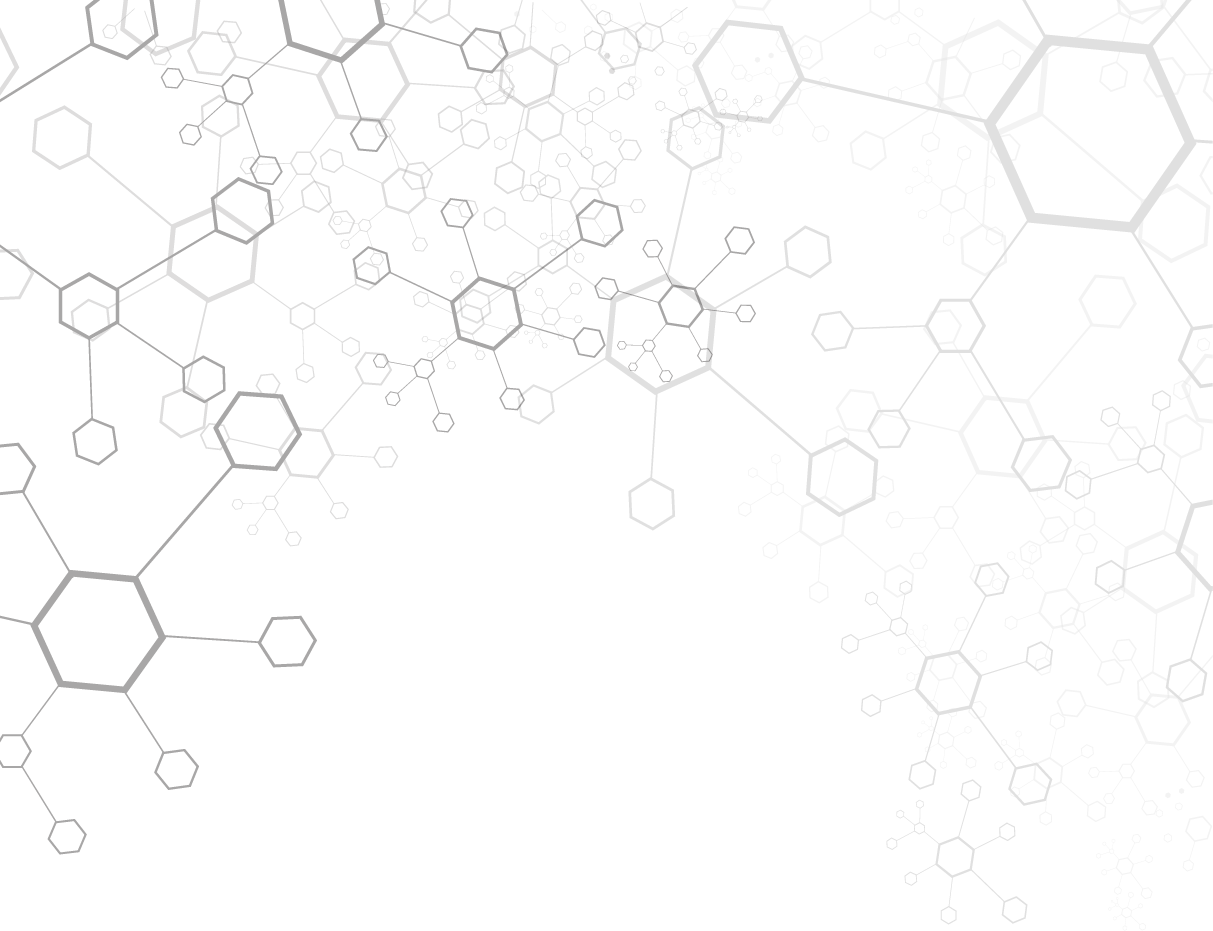
\includegraphics[width=\paperwidth,height=\paperheight]{moderncv/pngegg.png}};
  \end{tikzpicture}
\section{\textbf{Educational Background}}
\smallskip
\tlcventry{2017}{2015}{M Tech (Master In Technology) Computer Science (Biometrics)}{ITM University, Gwalior \emph{}}{Major in Computer Science}{In the Fieldsof Biometrics }{}

\smallskip

\tlcventry{2014}{2013}{PGDCA (Post Graduate Diploma In Computer Application)}{CPITM,Gwalior}{Makhanlal Chaturvedi Rashtriya Patrakarita Vishwavidyalaya, Bhopal \emph{}}{}{}{}
\smallskip

\tlcventry{2012}{2008}{BE (Bachelor of Engineering)}{Rajiv Gandhi Proudyogiki Vishwavidyalaya, Bhopal, MP\emph{}}{Major in Information Technology}{}
\smallskip
%\tlcventry{2008}{2007}{XII (PCM)}{\textbf{MP Board}, Bhopal\emph{}}{Math Stream}{Percent: \textbf{72}\%}
%\smallskip
%\tlcventry{2006}{2005}{X (Science)}{MP Board, Bhopal\emph{}}{Science Stream}{Percent: \textbf{75}\%}


%\section{\textbf{Theses}}
%\subsection{\textbf{M Tech Thesis}}

%\cvitem{\textbf{TITLE}}{A ROBUST METHOD TO RECOGNISE PALM VEIN USING SIFT \& SVM CLASSIFIER}

%\cvitem{\textbf{ADVISOR}}{Dr Vivek Singh}
%\cvitem{\textbf{FUNDING AGENGY}}{ITM University, Gwalior 
\smallskip

%\subsection{\textbf{PGDCA Project}}
%\cvitem{\textbf{TITLE}}{School Management System in Visual Basic  }
%\cvitem{\textbf{Description}}{This project can be used for some school academic and financial support like student records and fee management. This project is completely designed for school management task. Back-end is used as Microsoft Access.}

\smallskip 

%\subsection{\textbf{BE Major Project}}
%\cvitem{\textbf{TITLE}}{LED BASED GRAPHICS EQUALIZER }
%\cvitem{\textbf{Description}}{This project can be used for playing various music applications through LED graphics equalizer. This project can be used in means of entertainment projects as well as in houses to display music pitch to light up LED.}
%\cvitem{\textbf{ADVISORS}}{Professors A.K. Singh \& Shailesh Pandey}

\medskip

\section{\textbf{Research Projects}}
\subsection{\textbf{A ROBUST METHOD TO RECOGNISE PALM VEIN USING SIFT AND SVM CLASSIFIER}}

\tlcventry{2017}{2016}{The Study of the human identification and authentication system using palm vein and palm print}{}{}{}{}
\cvitem{\textbf{Description}}{This is my recently research work in the field of biometrics. This is also accepted in IJAST journal. This is a human identification system that simulate in MATLAB. I found performance measures up to 92 \%.}
\cvitem{\textbf{Toolbox}}{Image Processing Toolbox™}

\smallskip

\section{\textbf{Research Interests}}
\cvitem{\textbf{\footnotesize{Biometrics, Network and Server, Cloud}}}{    
    \begin{itemize}
    \item Biometric Human Identification System
    \item Manet, Vanet and WSN
%    \item Neural Network
    %\item Internet Of Things
   % \item AI and Neural Network
     %\item Sentimental analysis
    %\item Regular Expression for Input control Technologies and programming 
    \end{itemize}
    }

\section{\textbf{Affiliations}}
\subsection{Project Training \& Certification}

\cvitem{\footnotesize \textbf{Vocational Training}}{\textbf{Defense Research \& Development Establishment} (\textbf{DRDE}) \emph{} }
\cvitem{\textbf{Robotic Process Automation}}{\emph{\textbf{RPA Architect using UiPath RPA Tool}} \newline \textbf{UiPath} \textbf{}} 
\cvitem{\textbf{URL Link}}{\url{https://drive.google.com/file/d/1vJxvLYDknMxHp6ecDxGpwZj68W634zqn/view?usp=sharing}}
\cvitem{\textbf{Robotic Process Automation}}{\emph{\textbf{SAP Automation using UiPath RPA Tool}}
\smallskip
\newline \textbf{UiPath} \textbf{}} 
\cvitem{\textbf{URL Link}}{\url{https://drive.google.com/file/d/1GGY5VWDo8uA88jUYC-QCb8aAYTB2wsQW/view?usp=sharing}}
\cvitem{\textbf{DevOps  Certification}}{\emph{\textbf{DevOps Tools Training and Live Projects}}
\newline   \textbf{IBM} \textbf{}} 
\cvitem{\textbf{URL Link}}
{\url{https://www.credly.com/badges/66767381-b666-410b-9e23-db8f9a15308f/public_url}}
\cvitem{\textbf{DevSecOps   Essential  Certification}}{\emph{\textbf{DevSecOps road-map and strategy}}
\newline   \textbf{IBM} \textbf{}} 
\cvitem{\textbf{URL Link}}
{\url{https://www.credly.com/badges/522a8a25-a6f2-47d0-b6f7-59fafb692b76/public_url}}
%\section{Teaching Experience}
%\smallskip
%\subsection{Teaching Assistant}

%\tldatecventry{2013}{Topics on Desktop publisher and Networking}{In the field of Technical education having 3-year teaching experience as asst.professor in computer science at CPITM Gwalior}{}{}{}
%A detail oriented and hardworking professional with remarkable analytical, logical skills and expert in performing complex operations
%\smallskip

%\tldatecventry{2014}{M Tech VLSI  In Electronics Department}{Proficient in maintaining, Guidance and troubleshooting the computer system (hardware and software) and existing network operations having 3-year Lab Analyst experience in ITM UNIVERSITY Gwalior as a Lab Analyst in VLSI Design ECE.}{}{}{}%{SUPERVISOR Dr. Shyam akashe}



  
\section{\textbf{Projects Completed}}
\begin{tikzpicture}[remember picture, overlay]
  \node[opacity=0.14,inner sep=1pt] at (current page.center)
   {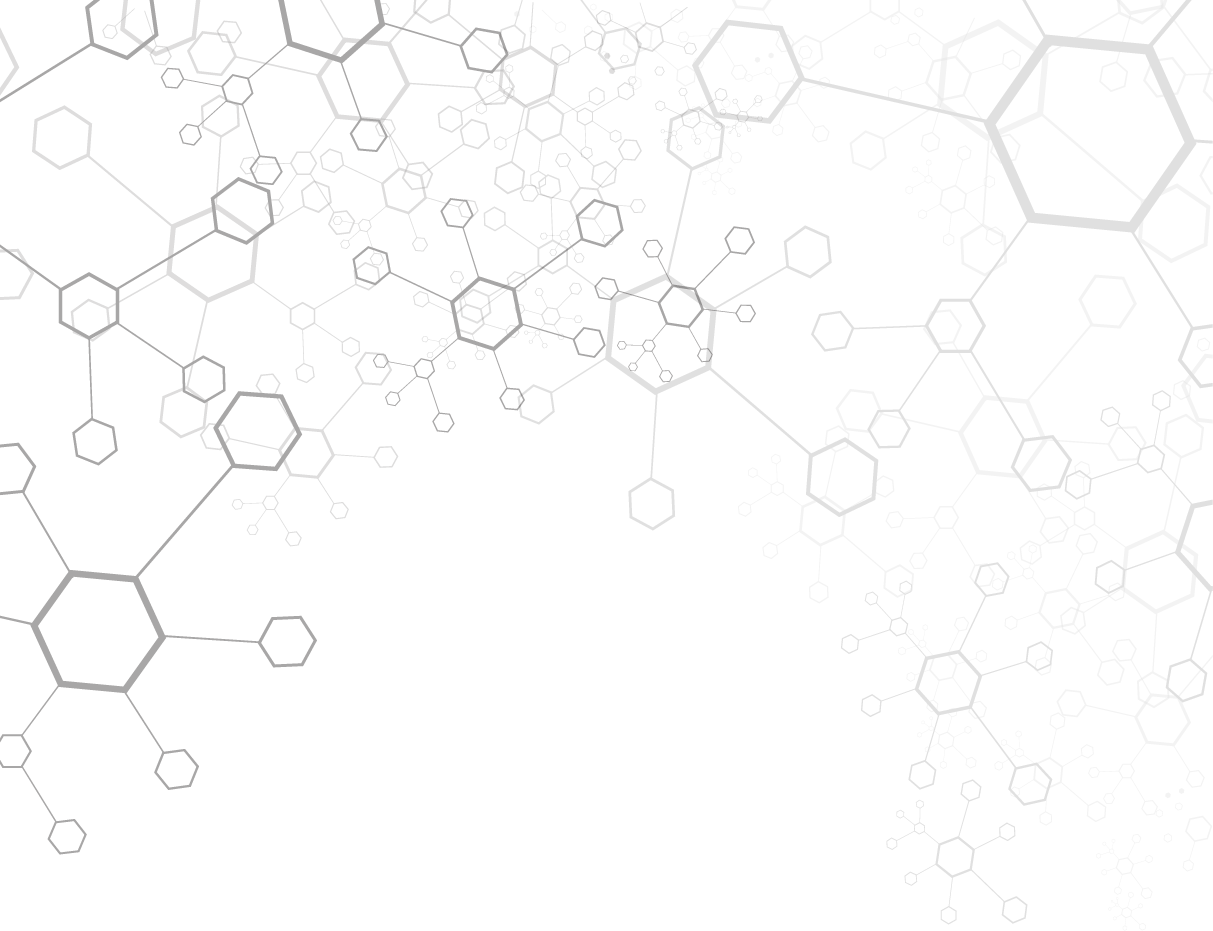
\includegraphics[width=\paperwidth,height=\paperheight]{moderncv/pngegg.png}};
  \end{tikzpicture}

  %Project8
  \smallskip
\tldatecventry{2023}{~ ~~\footnote[8]\textbf{Lead deployment and release automation efforts using Tekton and Argo CD on Red Hat OpenShift Cluster}}{}{\textbf{Hetrz Corp.}}{}{}
\cvitem{\textbf{Role}}{\textbf{Release Manager} }\cvitem{\textbf{Tools}}{IBM Cloud, AWS Production with openshift cluster, IBM container registry, TekTon CI and Argo CD, git, Openshift Cluster[GitOps] }

\cvitem{\textbf{Description}}{ Developed and deployed a custom end-to-end CI/CD solution for JAVA rental application frontend web and back-end services on Openshift Cluster. Utilized Tekton pipelines and Argo CD to automate the deployment process, ensuring fast and reliable releases. Implemented image protection using IBM Container Registry to safeguard sensitive images and maintain data integrity. Resulted in a secure and efficient deployment process, reducing manual intervention and enhancing application delivery speed. }
  \smallskip
  
  
  %Project7
  \smallskip
\tldatecventry{2022}{~ ~\footnote[7]\textbf{Data pipeline Automation(MLOps)}}{}{\textbf{Hertz Corp.}}{}{}
\cvitem{\textbf{Role}}{\textbf{DevSecOps Resource} }\cvitem{\textbf{Tools}}{AWS Cloud,Python,SQL data source,  Bitbucket, Jenkins(Bees), Databricks, and Airflow. }

\cvitem{\textbf{Description}}{ Designed and deployed a comprehensive, end-to-end data pipeline to streamline data processing and automation, leveraging Jenkins for continuous integration and delivery, Databricks for scalable data transformation, AWS Glue for ETL processes, and Apache Airflow for workflow orchestration. Enhanced data ingestion, transformation, and storage, significantly improving data quality and reducing processing time. Established monitoring and error-handling mechanisms to ensure reliability and scalability of the pipeline. Successfully delivered a robust, automated solution that enabled timely, accurate insights, driving data-driven decision-making across the organization. }
  \smallskip
  %Project6
  \smallskip
\tldatecventry{2021}{\footnote[6]\textbf{Custom CI-CD Management, Building and Deployment with Dev Support}}{}{\textbf{CISCO}}{}{}
\cvitem{\textbf{Role}}{\textbf{GCP DevOps Resource} }\cvitem{\textbf{Tools}}{GCP Cloud,Python,Snowflake Data Cloud,  Bitbucket, Jenkins(Bees), JFrog Artifactory, Spinnaker, Red Hat Quay, Git Hooks., SonarQube, Vault by HashiCorp. }

\cvitem{\textbf{Description}}{ This is the Custom CI-CD project for deployment of python back-end directly on GCP services like Cloud Run, Function,Spanner, Collection, K8 instances and storage etc. on single commit in SCM(GIT, Bitbucket etc.). This workflow provides automation for deployment of various packages. 
This CI- CD provides various functionalities like unit testing, code analysis and security governance also. Another responsibilities to manage, Build GCP Infra as required. }
\begin{figure}
\centering{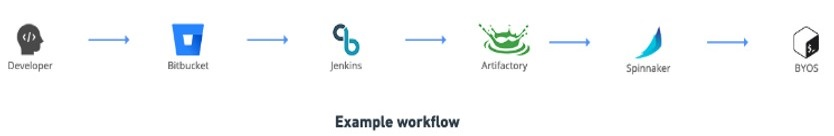
\includegraphics[height=2.57cm, width=18cm]{pipeline}}

\end{figure}

  
  
%project5
\smallskip
\tldatecventry{2021}{\footnote[5]\textbf{CentOs Web Panel/aapanel Deployment and Configuration for Ramjas College(Delhi University) with Azure Cloud}}{}{}{}{}
\cvitem{\textbf{Role}}{\textbf{Azure DevOps Resource/ Self} }\cvitem{\textbf{Tools}}{CentOS 8 VM On Azure Cloud}
\cvitem{\textbf{Description}}{ CWP/aapanel is a World Leading advanced Free and PRO web hosting panel that gives you all the flexibility to effectively and efficiently manage your server and clients. Now with CWP/aapanel Secure Kernel providing the highest possible security level for your server.Managing the whole panel for Ramjas Web project and Configure the various component like Domain Configuration and Security related Components. }

%project4
\smallskip
\tldatecventry{2020}{\footnote[4]\textbf{Deployment of ASP Dot Net Projects On Docker Container \& Kubernetes with Azure Cloud}}{}{}{}

\cvitem{\textbf{Role}}{\textbf{ARTP Support Engineer/ Self}}
\cvitem{\textbf{Tools}}{Docker,Kubernetes, Visual Studio, Mysql, Azure Cloud(AKE), Ubuntu 18.04(Linux Container) }

\cvitem{\textbf{Description}}{ HRMS Project developed in ASP Dot Net Core and Mysql. we have to create an container registry then create a service principal and configure its access to Azure resources (az ad sp create-for-rbac). Create AKS using node size and node count then deploy our asp project on Cluster using docker compose file and create service as load balancer in Azure to accessing the pods. }
%project 3
\smallskip
\tldatecventry{2019}{\footnote[3]\textbf{Deployment of PHP Projects (Wordpress and laravel) On Docker Container with AWS Cloud and On-Premises}}{}{}{}{}
\cvitem{\textbf{Role}}{\textbf{ARTP Support Engineer/ Self} }\cvitem{\textbf{Tools}}{Docker, Composer,Mysql,Nginx, AWS, Ubuntu 18.04 }
\cvitem{\textbf{Description}}{Electronic Time sheet Project developed in Laravel and Mysql. we have to create an container using docker composer file and configure thought ip \& port then map with nginx site configuration for pointing the domain}


\begin{tikzpicture}[remember picture, overlay]
  \node[opacity=0.14,inner sep=1pt] at (current page.center)
   {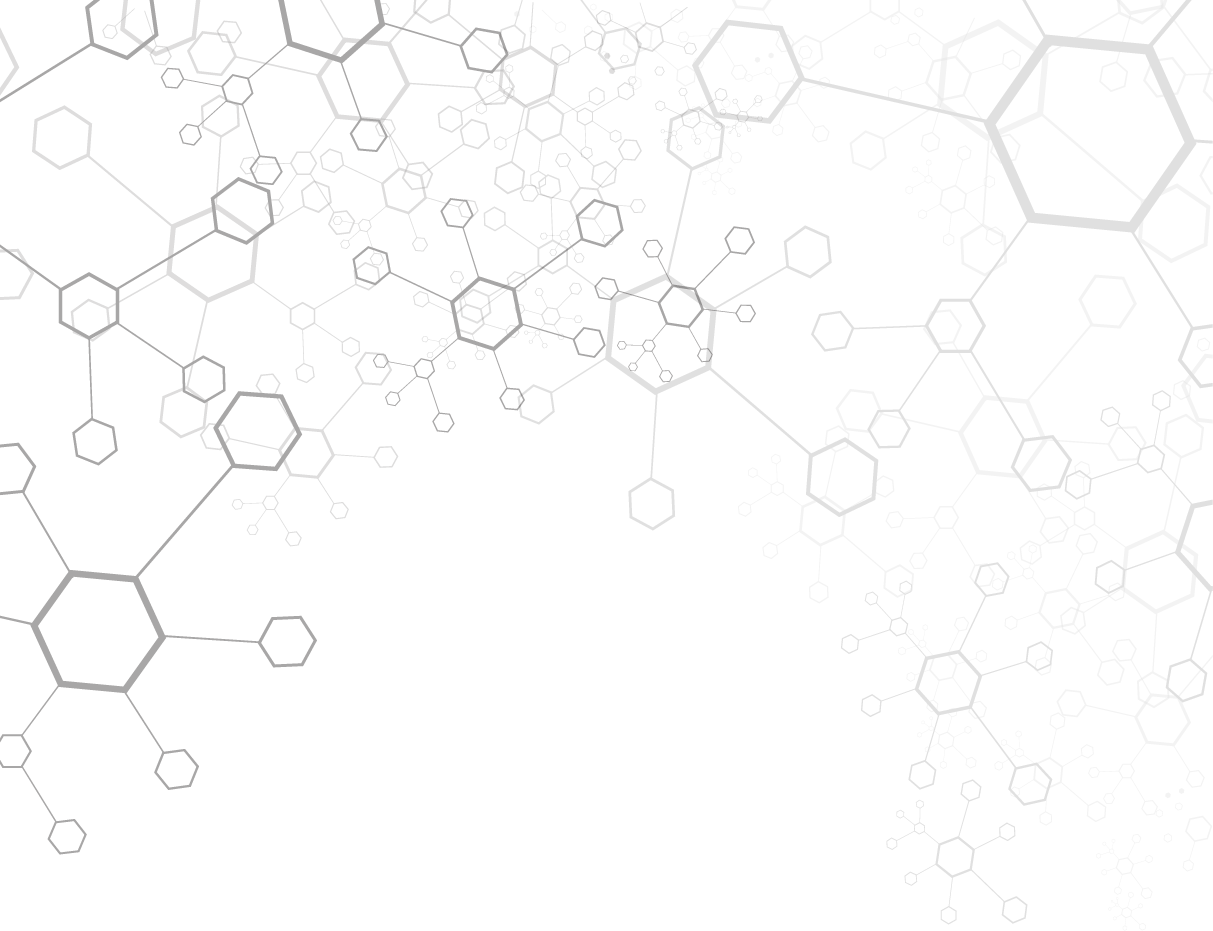
\includegraphics[width=\paperwidth,height=\paperheight]{moderncv/pngegg.png}};
  \end{tikzpicture}

%project 1
\smallskip
\tldatecventry{2018}{\footnote[2]\textbf{Setup Startup and Live Updater}}{}{}{}{}
\cvitem{\textbf{Role}}{\textbf{Software Engineer/ Self} }\cvitem{\textbf{Tools}}{Vb.Net, C\#, MVC(Basic Level),Web Api (Basic level),WPF(Basic level), MYSQL, DOS, PowerShell, SQL Server 2012(Intermediate), Crystal Report, Matlab (Image Processing Library) }
\cvitem{\textbf{Description}}{In this project automate the whole scenario of CBO Wholesale Retail Software. It’s configured the servers like MySQL, SQL 2012 and registered the Dll (Data Link Library) components of the project. This project common to all windows platforms.  }
\cvitem{\textbf{Problems/Needs}}{Software Installation and configuration on Windows So required custom installer package}
\cvitem{\textbf{Solutions / Objectives}}{This is the Automated software package that fulfill the all requirement of CBO Wholesale retail Software like SQL Server, Crystal Report and Other Dll.}
%project2

\tldatecventry{2017}{\footnote[1]\textbf{CBO W/R (Whole Sale Retail Software for Trading Purpose)}}{}{}{}{}
\cvitem{\textbf{Role}}{\textbf{Team Member}}
\cvitem{\textbf{Description}}{In this project target to end users they sale products and not belongs to ERP module. It is the complete trading software for Retalers, whole seller, stockiest, distributor's and so on.}

%\tldatecventry{2018}{\textbf{Help and Support Documentation and Notification Guide}}{}{}{}{}
%\cvitem{\textbf{Role}}{Software Engineer/ Self }
%\cvitem{\textbf{Description}}{In this project need more documentation for knowing about complete functionality of this software. So,help (*CHM) are required. CBO wholesale retail most of the time major changes so required the software update notification that completely designed in WPF and MVC framework.   }

%\tldatecventry{2019}{\textbf{Support and debugging, bug fix ware house management Software, CBO Software}}{}{}{}{}
%\cvitem{\textbf{Role}}{Software Support Engineer/ Self }
%\cvitem{\textbf{Description}}{Basically we get an exception/error during application execution at the level of database and OS based. We can resolve at database level as well as analysis of code at debugging level. We also done unit testing of software at various levels and further provides for UAT (User acceptance testing). report amendment at various levels (using SQL, Codes) according to user requirements.   }


%\cvitem{\textbf{SolutionReferences / Objectives}}{This is the support guide that fulfill the all requirement of CBO Wholesale retail Software.}
\section{\textbf{Academic Certificates Links}}
\cvitem{\textbf{Academic Certificates \& Documents}}{\url{https://drive.google.com/file/d/1tLz-RjWYRG6VdSd_8Orq4ESPjLeEVRaT/view?usp=sharing}}

\section{\textbf{Professional Certificates}}
\begin{figure}
\centering{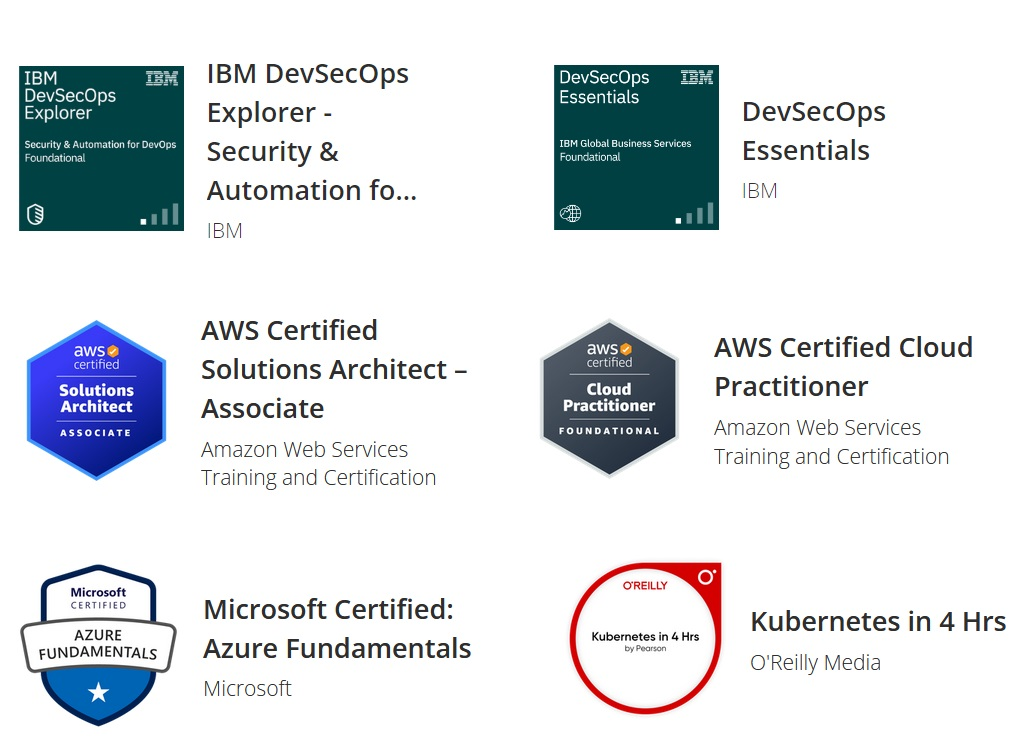
\includegraphics[height=10cm, width=20cm]{certificate.jpg}}

\end{figure}
\nocite{*}
\bibliographystyle{apalike}

\clearpage


\end{document}